\documentclass[12pt,dvipdfmx]{article}
\setlength{\oddsidemargin}{-1.3truecm}
\setlength{\evensidemargin}{-1.3truecm}
\setlength{\textwidth}{18.5truecm}
\setlength{\headsep}{1truecm}
\setlength{\topmargin}{-2truecm}
\setlength{\textheight}{24truecm}

\usepackage{graphicx}
\usepackage{listings}
\usepackage{fancybox}
\usepackage{hyperref}
\usepackage{color}

%%%%%%%%%%%%%%%%%%%%%%%%%%%
%%% define some colors for convenience
%%%%%%%%%%%%%%%%%%%%%%%%%%%

\newcommand{\mido}[1]{{\color{green}#1}}
\newcommand{\mura}[1]{{\color{purple}#1}}
\newcommand{\ore}[1]{{\color{orange}#1}}
\newcommand{\ao}[1]{{\color{blue}#1}}
\newcommand{\aka}[1]{{\color{red}#1}}

\lstset{language = C,
numbers = left,
numberstyle = {\tiny \emph},
numbersep = 10pt,
breaklines = true,
breakindent = 40pt,
frame = tlRB,
frameround = ffft,
framesep = 3pt,
rulesep = 1pt,
rulecolor = {\color{black}},
rulesepcolor = {\color{black}},
flexiblecolumns = true,
keepspaces = true,
basicstyle = \ttfamily,
identifierstyle = ,
commentstyle = ,
stringstyle = ,
showstringspaces = false,
tabsize = 4,
escapechar=\@,
}

\newcommand{\ubuntubutton}{Ubuntuボタン}

\renewcommand{\thesection}{問題\arabic{section}}

\title{問題}
\author{}
\date{}

\begin{document}
\maketitle

\section{}

\subsection{{\scriptsize 初めての物理シミュレーション}}
Visual Pythonを用いて,
投射角 $\theta$ で発射されたボールの軌道をアニメーションせよ.

\begin{enumerate}
\item まずは指定された角度で発射された一つのボールのアニメーションをせよ
\item ボールの軌跡が残るようにせよ(curveを用いる)
\item 角度を複数(リストで)与えられ,
  全ての角度で発射されたボールを同時にアニメーションせよ.
  余力があれば,全てのボールに違う色を付けてみよ.
\end{enumerate}

\begin{center}
\includegraphics[width=0.5\textwidth]{out/pdf/img/para.pdf}
\end{center}

\newpage

\iffalse
\section{}
2次関数 
\[ f(x) = a_2 x^2 + a_1 x + a_0 \]
が,$f(-1) = 1$, $f(1) = 3$, $f(2) = 7$を満たすとき,
$a_0, a_1, a_2$を求めよ,という問題は以下の連立一次方程式を解けば良い.

\[
\begin{array}{ccccccccc}
a_0 & + & (-1) & a_1 & + & (-1)^2 & a_2 & = & 1 \\
a_0 & + &   1  & a_1 & + & 1^2    & a_2 & = & 3 \\
a_0 & + &   2  & a_1 & + & 2^2    & a_2 & = & 7
\end{array}
\]

一般化して,$n$個の$x$座標$x_0, \ldots , x_{n-1}$と
$y$座標$y_0, \ldots , y_{n-1}$がそれぞれリストの形で与えられ,
\[ f(x_i) = y_i \; (i = 0, \ldots , n - 1) \]
を満たす$(n-1)$次多項式を求める関数{\tt find\_poly(X, Y)}を書け.

連立一次方程式を解くのに,numpyのlinalg.solveを用いるとよい.

$x, y$座標を乱数で与え,それらを通る多項式を求めてみよ.
求めたらそのグラフをmatplotlibを用いて表示せよ.
与えらた点も重ねて表示せよ.以下は4点を与えた(3次関数)
例でである.

\begin{center}
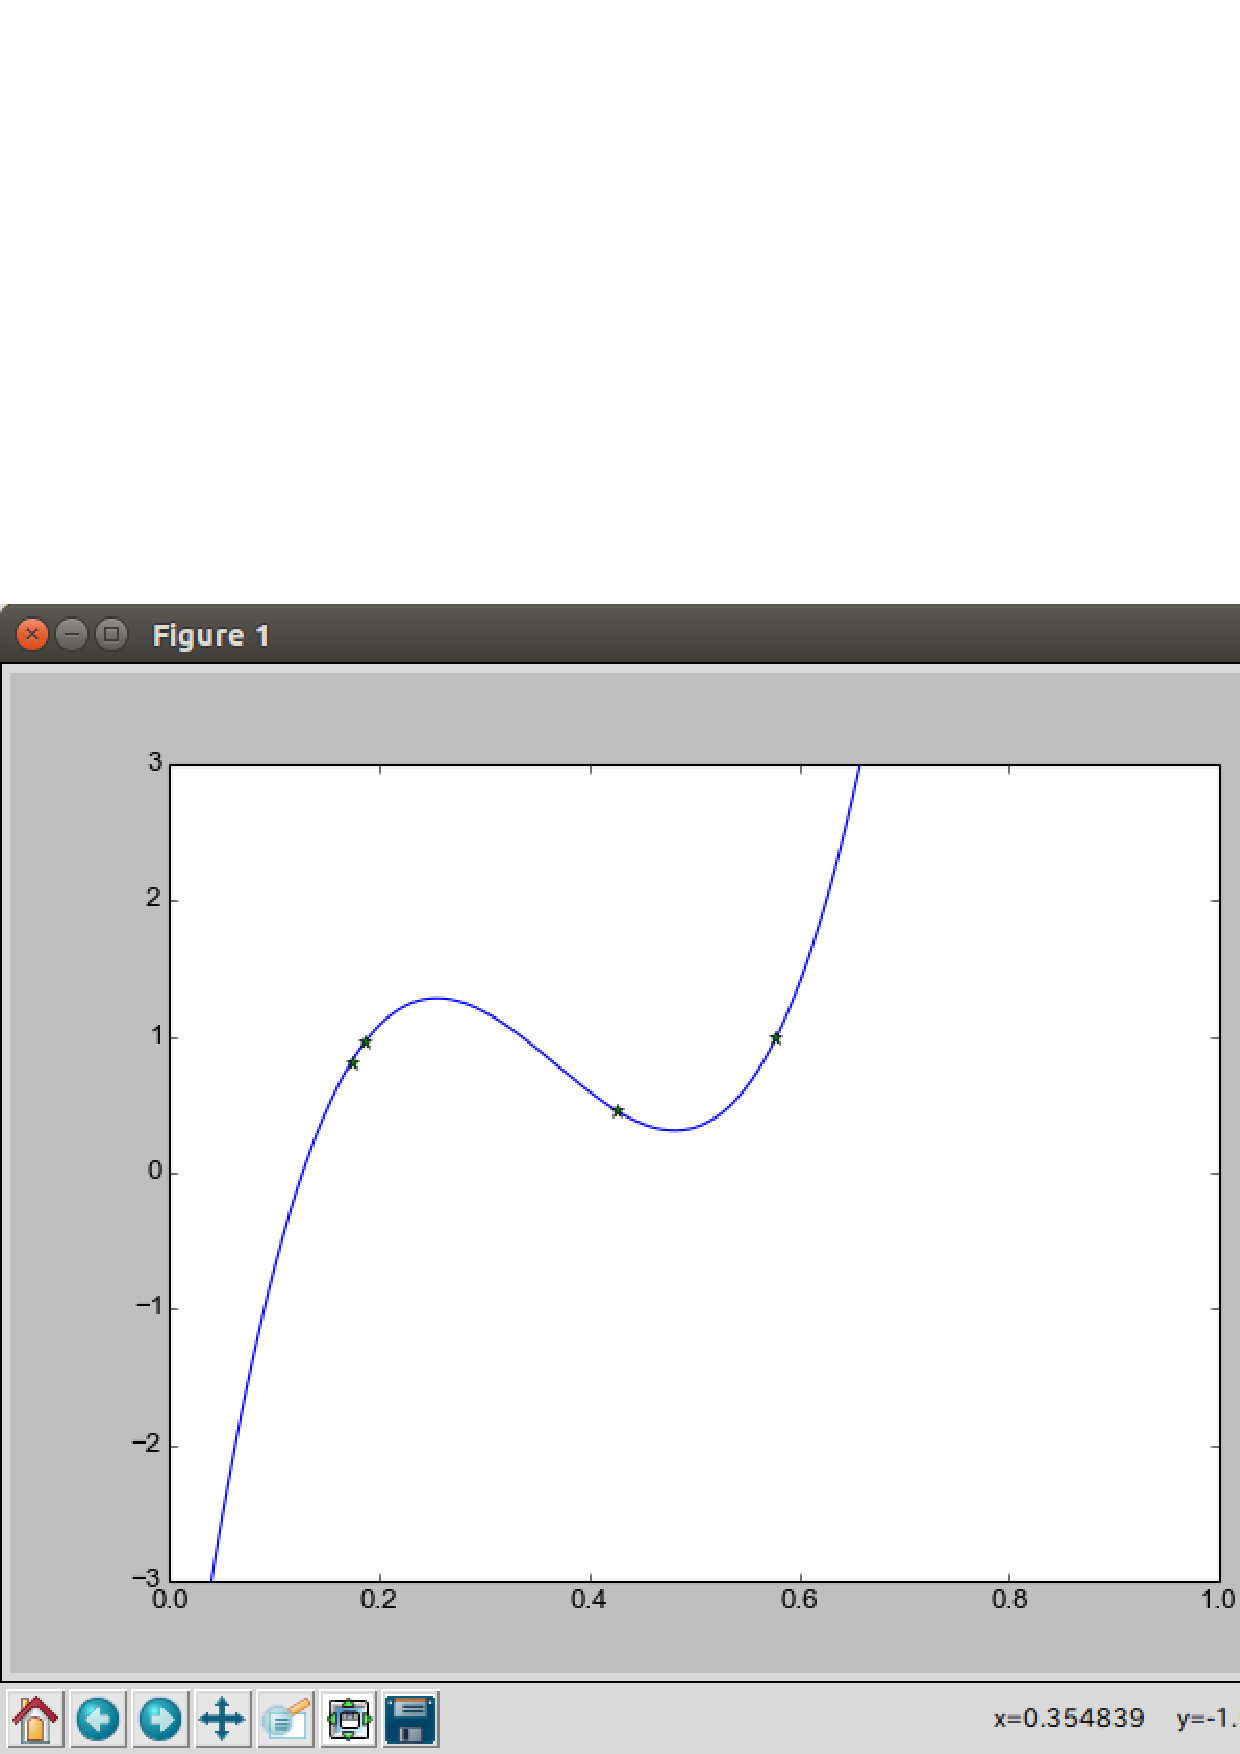
\includegraphics[width=0.5\textwidth]{out/pdf/img/poly.pdf}
\end{center}

\newpage
\fi



\section{}
\[ f(x,y) = x^2 + 2xy + 3y^2 + 4x + 5y \]
の,$[-10,10] \times [10,10]$における最小を求めよ.

なお,{\tt scipy.optimize} というモジュールにはその名もズバリ,
{\tt minimize}という関数がある.それを使う練習もした上で,
あえて自分でもやってみよ(いくつかやり方がある).

また,matplotlibを用いて$f(x, y)$のグラフを書け.
等高線表示({\tt contour}),色で表示({\tt pcolor}),
3次元の局面表示({\tt plot\_surface}),
枠線表示({\tt wire\_frame})などを試してみよ.

\section{}
領域$[0,1] \times [0,1]$の内部で
\[ \frac{\partial^2 f}{\partial x^2} + \frac{\partial^2 f}{\partial y^2} = 0 \]
を満たし,境界では以下のような値を取る$f$(の近似値)を求め,
結果を色表示してみよ.

\begin{enumerate}
\item $f(x, 0) = 0$, $f(x, 1) = 1$, $f(0, y) = f(1, y) = y$
\item $f(x, 0) = f(0, y) = 1 - x - y$, $f(x, 1) = f(1, y) = 0$
\end{enumerate}

この方程式(ラプラス方程式)は様々な現象で現れる.
なぜ,こうも異なる現象が似た方程式で現れるのかは不思議としか言いようがないのだが,
例えば,熱伝導率が一定の平面上での定常的な温度分布,
電荷がない空間での電位,質量がない空間での重力ポテンシャル,
非圧縮渦なしの流れの速度ポテンシャル($\nabla \phi = $速度となるような$\phi$),
などが上記を満たす.


\end{document}


